%--------------------------------------------------------------------------------
% Constrói a capa com base na seção de identificação do main.tex
%--------------------------------------------------------------------------------
\begin{capa}
    \setlength{\belowcaptionskip}{0pt}
    \setlength{\abovecaptionskip}{0pt}
    \setlength{\intextsep}{-18pt}
        \begin{figure}[h]
    		\begin{center}
    		    
\includegraphics[scale=1.0]{img/LOGO_UNIVASF_big.pdf}
    		\end{center}
    	\end{figure}

        %
\includegraphics[scale=0.6]{img/univasf.jpg}
        \center
    	{\ABNTEXchapterfont\large\imprimirinstituicao}

    	\vspace*{2cm}
    	    {\imprimirautor}
    	\vspace*{2cm}
    %	\vfill
        \begin{center}
    		\ABNTEXchapterfont\bfseries\large\imprimirtitulo
        \end{center}
    	\vfill

    	\ABNTEXchapterfont\bfseries\large\imprimirlocal\\ 
    	\the\year

    	\vspace*{1cm}
\end{capa}
%--------------------------------------------------------------------------------
% Constrói a folha de rosto com base na seção de identificação do main.tex
%--------------------------------------------------------------------------------
\begin{folhaderosto}
\center
    	{\ABNTEXchapterfont\large\imprimirinstituicao}

		\vspace*{2cm}
    	    {\imprimirautor}
    	\vspace*{2cm}
		\vspace*{\fill}

		{\ABNTEXchapterfont\bfseries\large\imprimirtitulo}
		\vspace*{\fill}

		{\hspace{.45\textwidth}
		\begin{minipage}{.5\textwidth}
			\SingleSpacing
			\imprimirpreambulo \\ \\

			{\imprimirorientadorRotulo~\imprimirorientador\par}
			{\imprimircoorientadorRotulo~\imprimircoorientador\par}

		\end{minipage}%
		\vspace*{\fill}}%
		\vspace*{\fill}
			\ABNTEXchapterfont\bfseries\large\imprimirlocal\\ 
			\the\year
		\vspace*{1cm}
\end{folhaderosto}

%--------------------------------------------------------------------------------
% Constrói a ficha catalográfia com base na seção de identificação do main.tex
% Está comentado porque no final das contas a biblioteca do seu campus que gera a 
% numeração, você pode adicionar os numeros aqui, ou anexar o pdf gerado por eles
% ao documento.
%--------------------------------------------------------------------------------
%\begin{fichacatalografica}
%	\vspace*{\fill}					% Posição vertical
%	\hrule							% Linha horizontal
%	\begin{center}					% Minipage Centralizado
%	\begin{minipage}[c]{12.5cm}		% Largura
%
%	\imprimirautor
%
%	\hspace{0.5cm} \imprimirtitulo  / \imprimirautor. --
%	\imprimirlocal, \the\year-
%
%	\hspace{0.5cm} xx p. : il. (algumas color.) ; 30 cm.\\
%
%	\hspace{0.5cm} \imprimirorientadorRotulo~\imprimirorientador\\
%
%	\hspace{0.5cm}
%	\parbox[t]{\textwidth}{\imprimirtipotrabalho~--~\imprimirinstituicao,
%	\the\year.}\\
%
%	\hspace{0.5cm}
%		1. Palavra-chave1.
%		2. Palavra-chave2.
%		I. Orientador.
%		II. Universidade xxx.
%		III. Faculdade de xxx.
%		IV. Título\\
%
%	\hspace{8.75cm} CDU 02:141:005.7\\
%
%	\end{minipage}
%	\end{center}
%	\hrule
%\end{fichacatalografica}

%--------------------------------------------------------------------------------
% Anexando a ficha catalogáfica e a folha de aprovação 
%--------------------------------------------------------------------------------
%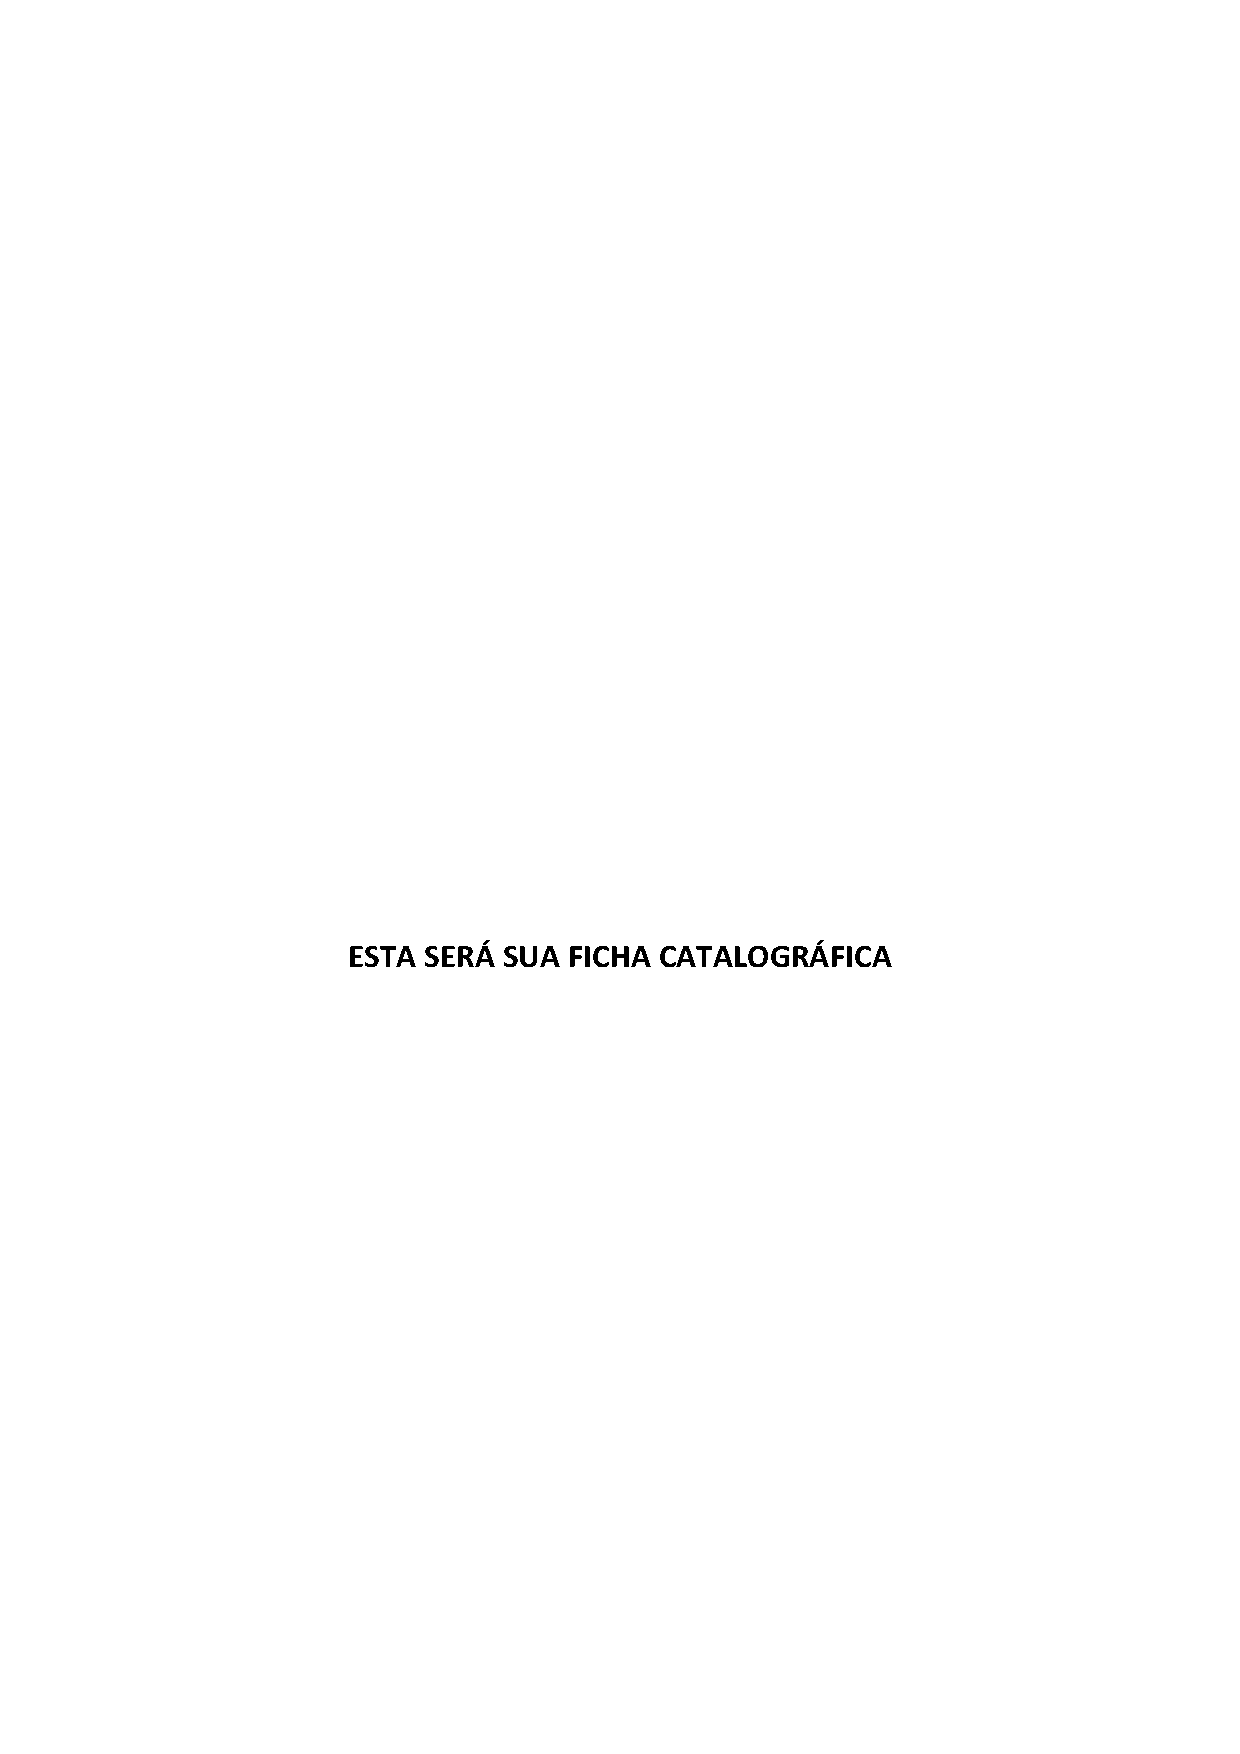
\includepdf[pages=-]{anexos/ficha.pdf}

%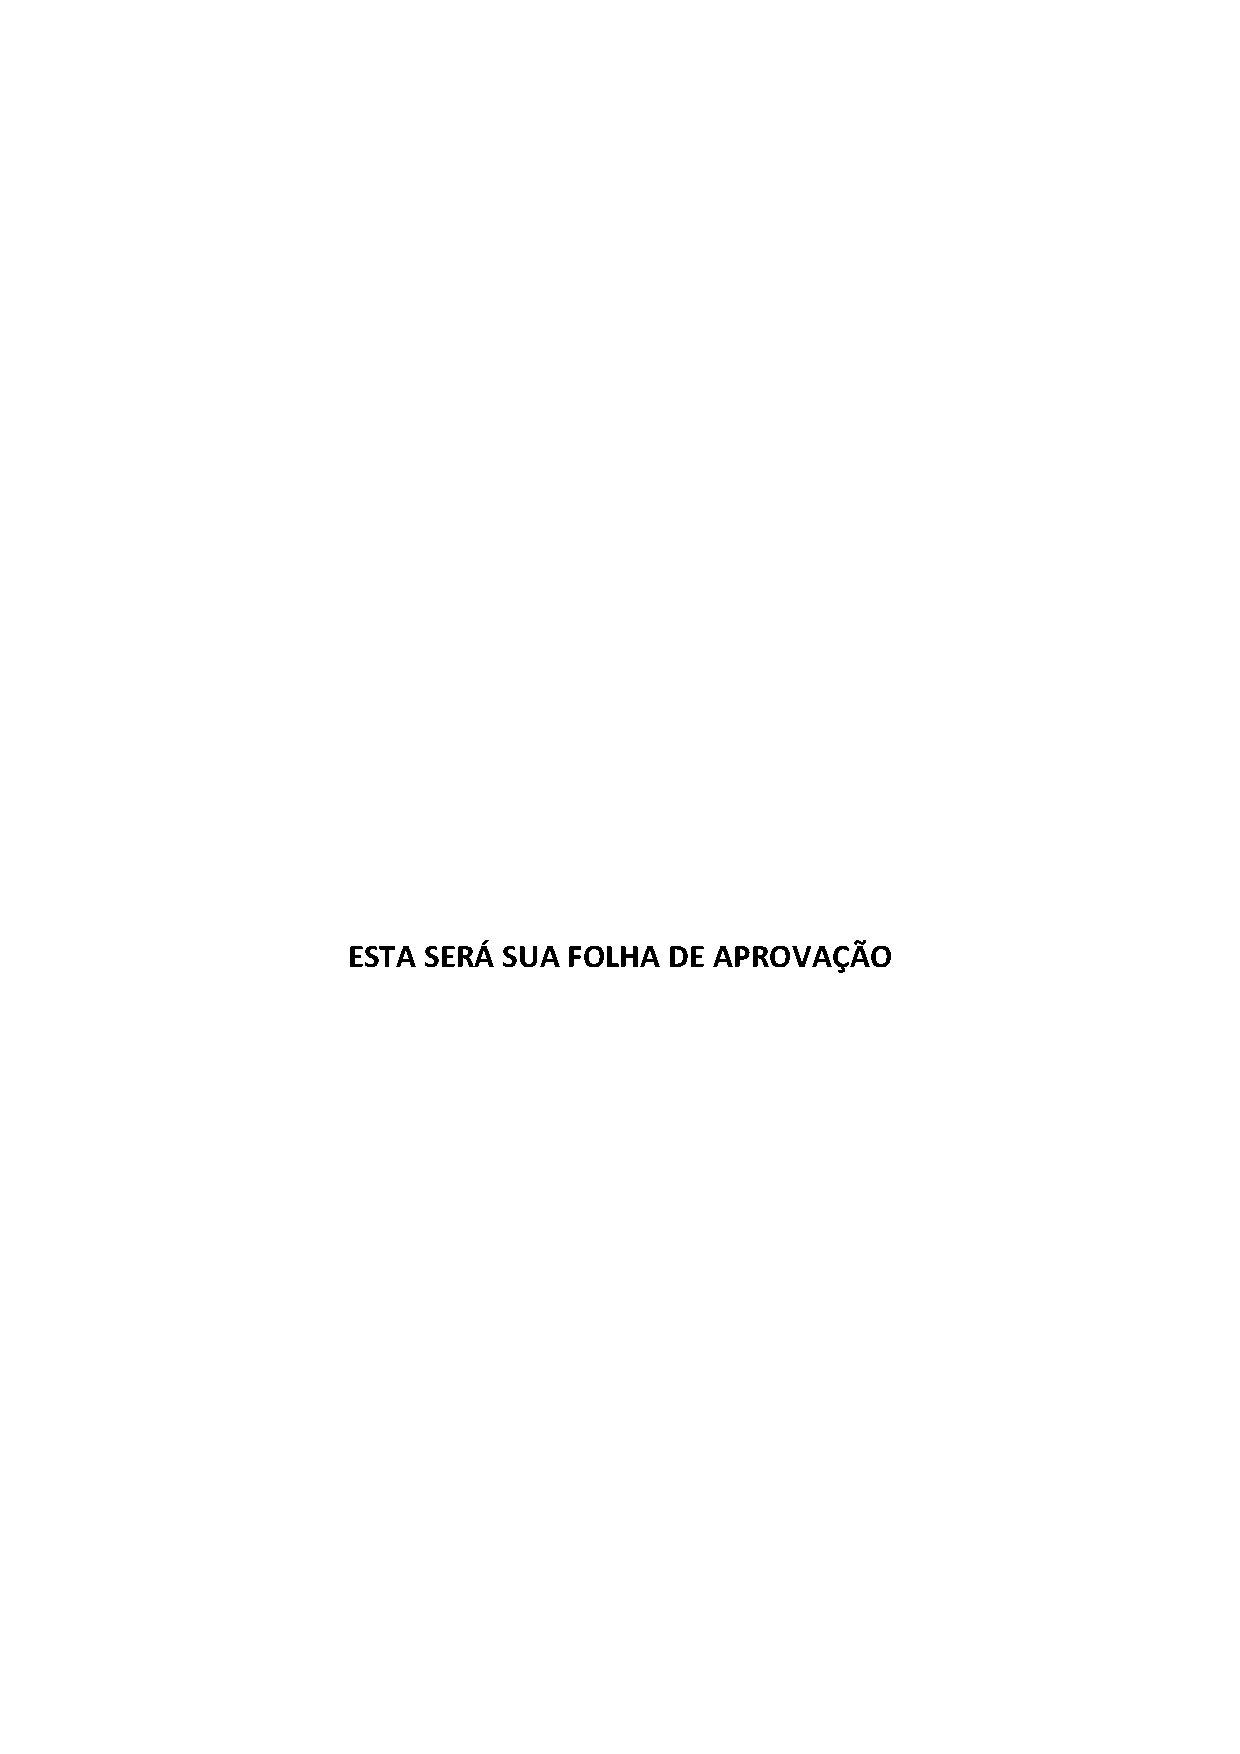
\includepdf[pages=-]{anexos/aprovacao.pdf}

\setlength{\ABNTEXsignwidth}{12cm}

%--------------------------------------------------------------------------------
% Está comentado pelo mesmo motivo da ficha catalográfica 
%--------------------------------------------------------------------------------
% \begin{folhadeaprovacao}
% 	\begin{center}
% 	    {\ABNTEXchapterfont\bfseries\large\imprimirinstituicao}
% 	    \vspace*{\fill}

% 	    {\ABNTEXchapterfont\bfseries\large FOLHA DE APROVAÇÃO}
% 	    \vspace*{\fill}

% 	    {\ABNTEXchapterfont\bfseries\large\imprimirautor}

% 	    \vspace*{\fill}\vspace*{\fill}
% 	    {\ABNTEXchapterfont\bfseries\large\imprimirtitulo}
% 	    \vspace*{\fill}

% 	    {\hspace{.45\textwidth}
% 		\begin{minipage}{.5\textwidth}
% 			\SingleSpacing
% 			\ABNTEXchapterfont\imprimirpreambulo \\ \\

% 			{\ABNTEXchapterfont\imprimirorientadorRotulo~\imprimirorientador\par}
% 			{\ABNTEXchapterfont\imprimircoorientadorRotulo~\imprimircoorientador\par}

% 		\end{minipage}%
% 	    \vspace*{\fill}}
% 	\end{center}

% 	\vspace*{\fill}

% 	\begin{center}
% 			 \ABNTEXchapterfont\large Aprovado em: \_\_\_\_ de \_\_\_\_ de 2019
% 	\end{center}

% 	\vspace*{\fill}

% 	\begin{center}
% 			 \ABNTEXchapterfont\bfseries\large Banca Examinadora
% 	\end{center}

%   \ABNTEXchapterfont\assinatura{Rosalvo Ferreira de Oliveira, Doutor, Universidade Federal do Vale do São Francisco}
% 	\ABNTEXchapterfont\assinatura{Jorge Luis Cavalcanti Ramos, Doutor, Universidade Federal do vale do São Francisco}
%  \ABNTEXchapterfont\assinatura{Ricardo Argenton Ramos, Doutor, Universidade Federal do Vale do São Francisco}
% 	 \vspace*{\fill}


% \end{folhadeaprovacao}

%--------------------------------------------------------------------------------
% Insere a epígrafe
%--------------------------------------------------------------------------------
\newpage
\begin{epigrafe}
\vspace*{\fill}
\begin{flushright}
		\textit{Planet Earth is blue and there's nothing I can do}\\
		\textbf{David Bowie}\\
		\textbf{Space Oddity}
\end{flushright}
\end{epigrafe}
%--------------------------------------------------------------------------------
% Seção de agradecimentos
%--------------------------------------------------------------------------------
\begin{agradecimentos}
	
Agradeço primeiramente a Deus e a minha família, principalmente meus pais, João
Alves e Regina Coeli, e a meus irmãos, Maria Alice e Luciano, pelo apoio e carinho
durante todo o caminho da graduação.

À minha noiva, Nathanaele, por mesmo longe se fazer presente e me incentivar a
continuar em frente sempre.

Agradeço ao ``Clubinho Guaraná'' composto por Ellen, Daniel, Talita, Carolina,
Isaac, Esron e Mauricio, pelos momentos compartilhados de alegria, estresse e,
as vezes, tristeza. Um grupo não só de leitura, mas de colaboração mútua e
respeito. Um agradecimento especial a Ellen por estar comigo desde o começo da
jornada.

Agradeço a meu orientador, Rosalvo, por me apresentar a oportunidade de dar
inicio ao projeto FutVasf2D e trabalhando comigo por 2 anos seguidos até
finalmente a conclusão.

Obrigado aos professores Ricardo Ramos e Jorge Cavalcanti que contribuíram com a
melhoria deste trabalho.

Obrigado ainda a Brauliro e Ricardo, novamente, com conselhos profissionais e
acadêmicos que contribuíram para formação e ofereceram momentos de lazer que se mostraram
um óasis em meio a todo o estresse do curso, se tornando amigos, ouso dizer.

Obrigado à Deise por sempre ajudar com toda a burocracia da UNIVASF, até quando
parecia que não tinha jeito.

Por fim agradeço a todos que estiveram comigo neste caminho, professores,
colegas e amigos. Obrigado por me ajudar a me tornar quem eu sou hoje.

\end{agradecimentos}

%--------------------------------------------------------------------------------
% Insere a segunda epígrafe
%--------------------------------------------------------------------------------
% \begin{epigrafe}
%     \vspace*{\fill}
% 	\begin{flushright}
% 		Se pude enxergar a tão grande distância, foi subindo nos ombros de gigantes.\\
% 		 \vspace{\baselineskip}
% 		\textbf{Isaac Newton}\\
% 		\textbf{Carta à Robert Hooke, 1676}
% 	\end{flushright}
% \end{epigrafe}



%--------------------------------------------------------------------------------
% Seção de resumos
%--------------------------------------------------------------------------------
% resumo em português
\setlength{\absparsep}{18pt} % ajusta o espaçamento dos parágrafos do resumo
\begin{resumo}

% Em geral o resumo precisa das seguintes partes [contexto], [problema],
% [solução/objetivo], [metodologia], [validação/experimento] e [resultados].

Este trabalho se debruça sobre a copa do mundo de futebol de robôs
(\textit{RoboCup Soccer}), que incentiva a produção de pesquisas na área de
inteligência artificial e robótica, enquanto parte do projeto FutVasf2D que
busca o desenvolvimento de um time oficial de futebol de robôs na liga de
simulação 2D para UNIVASF, investigando o efeito de diferentes modelos
de mundo aplicados à técnica de aprendizado por reforço \textit{Q-Learning}
sobre a performance do time na posição de defesa. Este trabalho busca encontrar
modelos que facilitem o aprendizado dos agentes na tentativa de interceptar
bolas lançadas pelo adversário e de capturar a bola em posse do adversário. Para
alcançar o objetivo foram desenvolvidos modelos através de diferentes
combinações de estados, ações, recompensas e métodos de implementação. Os
modelos foram treinados e avaliados através da ferramenta HFO que cria situações
de defesas aleatoriamente agilizando o processo de treinamento. Os resultados
encontrados foram comparados entre si e entre o time base original
(\textit{WrightEagleBASE}), mas apresentaram desempenho abaixo do esperado,
levando discussões de possíveis falhas no processo.


 \textbf{Palavras-chave}: Futebol de Robôs, Aprendizado por reforço, \textit{Q-Learning}, \textit{RoboCup Simulation 2D}, Defesa.

\end{resumo}

%---------------------------------------------------------------------------------
% resumo em inglês
\begin{resumo}[Abstract]
\begin{otherlanguage*}{english}

	This work dwell on the soccer world cup (RoboCup Soccer), which encourages
	researchers in the artificial intelligence and robotics fields, being part
	of the FutVasf2D project that looks for the development of an official robot
	soccer team in the 2d simulation league to the UNIVASF, investigating the
	effects of different world designs applied to the reinforcement technique
	Q-Learning about the performance of the team in defense position. This work
	tries to find designs that improve the learning of the agents into trying to
	intercept balls launched by the adversaries and capture the ball in the
	opponent possession. To reach this objective designs with differents
	combination of states, actions, rewards and implementation methods were
	developed. The designs were trained e evaluated through the HFO tools, which
	creates situations of defense randomly making the learning process faster.
	The found results were compared between themselves and the original base
	team (WrightEagleBASE), but showed performance below the expected, leading
	to discussions about the possible faults in the process.
	
	\vspace{\onelineskip}

	\noindent
	\textbf{Key-words}: \textit{Robot Soccer, Reinforcement Learning, Q-Learning, RoboCup Simulation 2D, Defense}.

\end{otherlanguage*}
\end{resumo}


%---------------------------------------------------------------------------------
% Insere lista de ilustrações
%---------------------------------------------------------------------------------
\begin{KeepFromToc} % Este comando evita que todas as seções dentro dele de apareçam no sumário
\pdfbookmark[0]{\listfigurename}{lof}
\listoffigures
%\addcontentsline{toc}{chapter}{Lista de Figuras}
\cleardoublepage


%---------------------------------------------------------------------------------
% Insere lista de tabelas
%---------------------------------------------------------------------------------
\pdfbookmark[0]{\listtablename}{lot}
\listoftables
\cleardoublepage

%---------------------------------------------------------------------------------
% Ajusta lista de código - alterar de figures para códigos - by @Gabrielr2508
%---------------------------------------------------------------------------------
\makeatletter
\let\l@listing\l@figure
\def\newfloat@listoflisting@hook{\let\figurename\listingname}
\makeatother

%---------------------------------------------------------------------------------
% Insere lista de códigos - by @leolleocomp
%---------------------------------------------------------------------------------
\listoflistings

\end{KeepFromToc}

%---------------------------------------------------------------------------------
% Insere lista de abreviaturas e siglas
%---------------------------------------------------------------------------------
\begin{siglas}
	\item[CBR] Competição Brasileira de Robótica
    \item[CMAC] Computador Aritmético de Modelo Cerebelar
    \item[DCBD] Descoberta de Conhecimento em Base de Dados 
    \item[HAQL] \textit{Q-Learning} Acelerado Heuristicamente
    \item[HFO] Ofensa de Meio Campo
    \item[KDD] Descoberta de Conhecimento em Base de Dados, do inglês \textit{Knowledge Discovery in Databases}
    \item[MDP] Processo de Decisão Markoviano
    \item[PIBIC] Programa Institucional de Bolsas de Iniciação Científica 
    \item[QRL] Aprendizado por Reforço Qualitativo
    \item[QSR] Raciocínio Espacial Qualitativo
    \item[RPROP] \textit{Backpropagation} Resiliente
    \item[SARSA] Estado-Ação-Recompensa-Estado-Ação
    \item[UNIVASF] Universidade Federal do Vale do São Francisco
	    
\end{siglas}

%---------------------------------------------------------------------------------
% Insere o sumario
%---------------------------------------------------------------------------------
\pdfbookmark[0]{\contentsname}{toc} 
\tableofcontents*
\cleardoublepage
